\documentclass[tikz,border=5pt]{standalone}
\usepackage{times}
\usepackage{amsmath,amssymb}
\usetikzlibrary{positioning,fit,arrows.meta,backgrounds,shapes.geometric,calc,shadows,decorations.pathreplacing}

\begin{document}
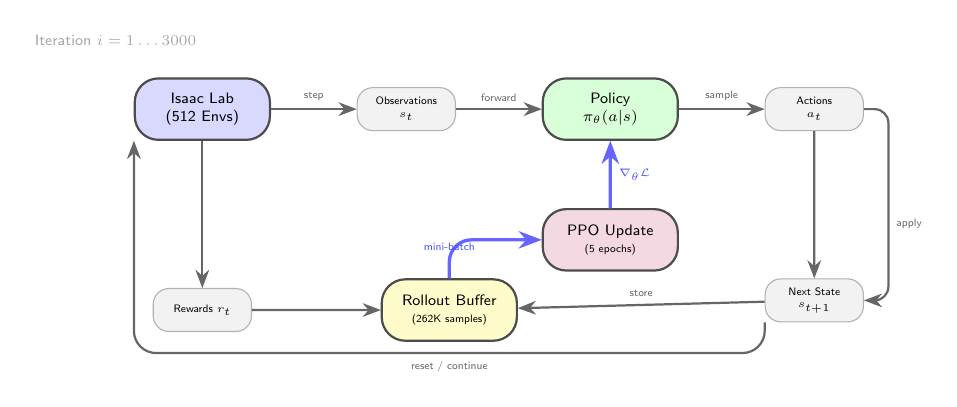
\begin{tikzpicture}[
    scale=0.78,
    transform shape,
    node distance=0.8cm,
    component/.style={
        draw=black!70,
        rounded corners=3mm,
        minimum width=2.2cm,
        minimum height=1cm,
        font=\sffamily\scriptsize,
        thick,
        align=center
    },
    data/.style={
        draw=gray!60,
        fill=gray!10,
        rounded corners=2mm,
        minimum width=1.6cm,
        minimum height=0.7cm,
        font=\sffamily\tiny,
        align=center
    },
    arrow/.style={->, >=Stealth, thick, color=black!60},
    bluearrow/.style={->, >=Stealth, very thick, color=blue!60}
]

% Top row - main forward pass
\node[component, fill=blue!15] (env) {Isaac Lab\\(512 Envs)};
\node[data, right=1.4cm of env] (obs) {Observations\\$s_t$};
\node[component, fill=green!15, right=1.4cm of obs] (policy) {Policy\\$\pi_\theta(a|s)$};
\node[data, right=1.4cm of policy] (actions) {Actions\\$a_t$};

% Middle row - PPO Update (raised to avoid overlapping arrows)
\node[component, fill=purple!15, below=1.1cm of policy] (update) {PPO Update\\{\tiny (5 epochs)}};

% Bottom row - data collection (buffer shifted right for better spacing)
\node[data, below=2.4cm of env] (rewards) {Rewards $r_t$};
\node[component, fill=yellow!20, below=2.4cm of obs, xshift=0.7cm] (buffer) {Rollout Buffer\\{\tiny (262K samples)}};
\node[data, below=2.4cm of actions] (next) {Next State\\$s_{t+1}$};

% Forward arrows (top)
\draw[arrow] (env) -- node[above, font=\sffamily\tiny] {step} (obs);
\draw[arrow] (obs) -- node[above, font=\sffamily\tiny] {forward} (policy);
\draw[arrow] (policy) -- node[above, font=\sffamily\tiny] {sample} (actions);

% Down arrows from top to bottom
\draw[arrow] (env.south) -- (rewards.north);
\draw[arrow] (actions.south) -- (next.north);

% Bottom flow: rewards and next state feed into buffer (straight arrows)
\draw[arrow] (rewards) -- (buffer);
\draw[arrow] (next) -- node[above, font=\sffamily\tiny] {store} (buffer);

% Mini-batch arrow: from buffer top, curves to PPO update left side
\draw[bluearrow, rounded corners=8pt] (buffer.north) |- node[above, font=\sffamily\tiny, color=blue!70, pos=0.25] {mini-batch} (update.west);

% Gradient update arrow: PPO update up to policy
\draw[bluearrow] (update.north) -- node[right, font=\sffamily\tiny, color=blue!70] {$\nabla_\theta \mathcal{L}$} (policy.south);

% Loop back arrow (starts from next.south west to avoid overlap)
\draw[arrow, rounded corners=8pt] (next.south west) -- ++(0,-0.5) -| node[below, font=\sffamily\tiny, pos=0.25] {reset / continue} (env.south west);

% Apply arrow on right side
\draw[arrow, rounded corners=5pt] (actions.east) -- ++(0.4,0) |- node[right, font=\sffamily\tiny, pos=0.3] {apply} (next.east);

% Title annotation
\node[font=\sffamily\scriptsize, color=gray!70, anchor=south] at ($(env.north west) + (-0.3, 0.4)$) {Iteration $i = 1 \ldots 3000$};

\end{tikzpicture}
\end{document}
